% die Standard-Dokumentenklasse
\documentclass[11pt,a4paper]{article} %% 1.Ebene = chapter, headings

% input encoding, font encoding, outline font
\usepackage[utf8]{inputenc} 
\usepackage[T1]{fontenc} 
\usepackage{lmodern}
\usepackage{tcolorbox}
% Sprache
\usepackage[german]{babel}

% Absatzformatierung
\setlength{\parindent}{0pt}
\setlength{\parskip}{1ex plus 0.5ex minus 0.5ex}

% erweiterte mathematische Symbole
\usepackage{amsmath} 

% für Abbildungen
\usepackage{graphicx} 

% für Tabellen
\usepackage{booktabs}

% für Hyperlinks
\usepackage[colorlinks]{hyperref}
\graphicspath{}

%%%%%%%%%%%%%%%%%%%%%%%%%%%%%%%%%%%%%%%%%
\begin{document}


{
	\centering 
	\large 
	Physiklabor für Anfänger*innen \\
	Ferienpraktikum im Sommersemester 2018 \\[4mm]
	\textbf{\LARGE 
		Versuch 4: Dichte und Oberflächenspannung
	} \\[3mm]
	(durchgeführt am 07.09.2018 bei Daniel Bartle) \\
	Ye Joon Kim, Marouan Zouari\\
	\today \\[10mm]
}

\tableofcontents
\section{Einleitung}
Zwei Methode, um die Dichte eines Objekts zu bestimmen, sind beispielsweise eine Jolly'sche Federwaage anzuwenden, oder direkt das Volumen und die Masse des jeweiligen Objekts zu messen. In dem ersten Versuchsteil werden beide Methode benutzt und verglichen. In dem 2. Versuchsteil wird die Oberflächenspannung, eine Quantifizierung der Kohäsion, von mehreren Flüssigkeiten bestimmt. 
\section{Ziel des Versuchs}
Das Ziel des ersten Teils des Versuchs ist es, die Dichte von festen Körpern und Flüssigkeiten zu bestimmen und beide Methodologien (beschrieben in Einleitung) zu vergleichen. Das Ziel des zweiten Teils ist es, die Oberflächenspannungen von Flüssigkeiten, nämlich von Wasser und Äthanol, zu bestimmen. 

\section{Aufbau}
Der Aufbau zum ersten Versuchsteil besteht aus einem Feder, zwei Waagschalen, einem Becher mit Flüssigkeit und einem vertikal verschiebbaren Tisch. 

In dem Zweiten Teil wurde ein Torsionkraftmesser verwendet. Auf einer Seite steht ein vertikal verschiebbarer Tisch, dessen höhe mit der Millimeterschraube abgelesen werden konnte. Auf dem Tisch lag ein mit einer Flüssigkeit gefüllter Becher wo das Drahtbügel eingetaucht werden konnte. 


\begin{figure}
	\centering
	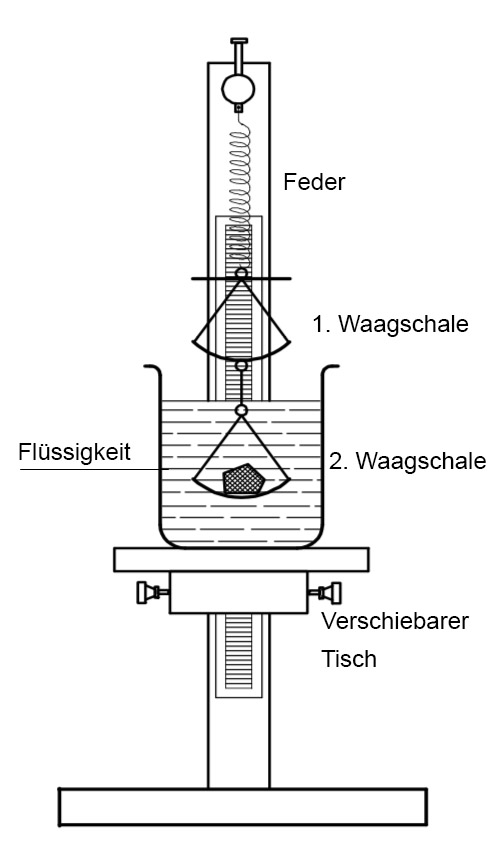
\includegraphics[scale=0.5]{Abb1}
	\caption{Aufbau zum 1. Versuchsteil. Eine Jollysche Federwaage. ("Versuchsanleitungen zum Physiklabor")}
	
	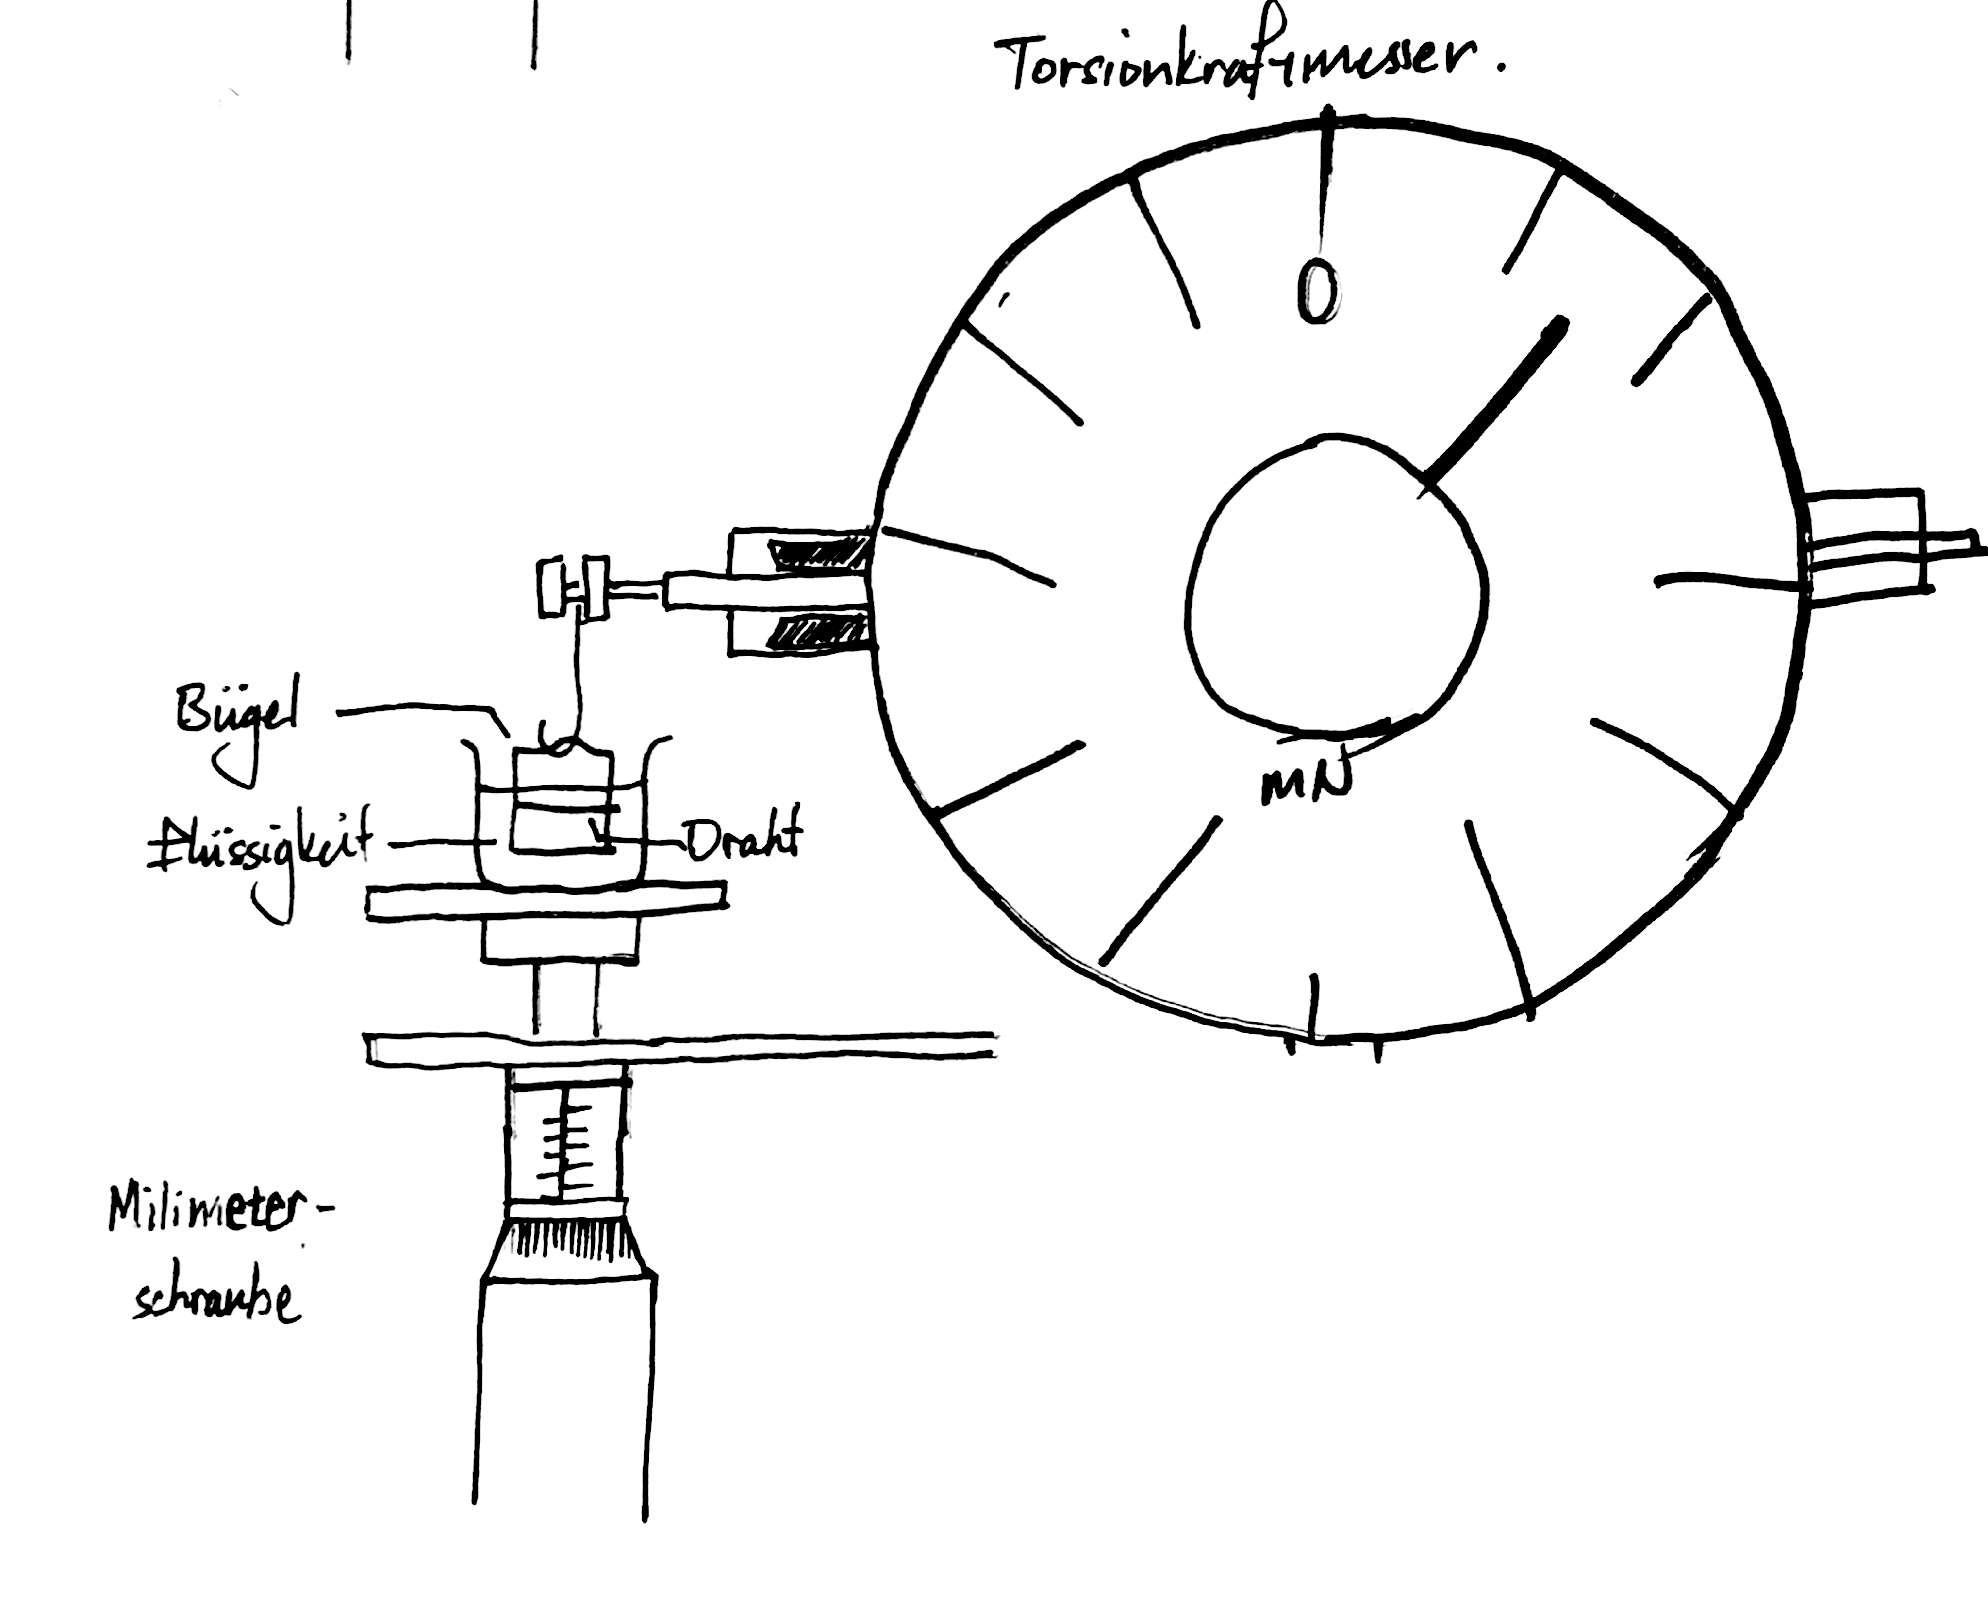
\includegraphics[scale=0.15]{Abb2}
	\caption{Aufbau zum 2. Versuchstail}
\end{figure}
\newpage

\section{Versuchsdurchführung}
Im ersten Teil wurden die geometrischen Abmessungen des Körpers mit einem Messschieber gemessen. Danach wurde ein Becher mit Wasser gefüllt und auf den Verschiebbaren Tisch gestellt. Danach wurden die Waagschalen an die Feder aufgehängt, sodass nur eine der Waagschalen in dem Flüssigkeit eingetaucht war. Der Körper wurde zuerst auf eine Waagschale gestellt. Die Auslenkung wurde mit dem horizontalen Teil oberhalb der ersten Waagschale gemessen. Es wurde mit dem Spiegel hinter der Skala sichergestellt, dass es keinen Parallaxefehler gab. Der Körper wurde getrocknet, falls nass, und dann auf die andere Waagschale gestellt. Die Auslenkung wurde wie vorher abgelesen. Dieser Prozess wurde für fünf unterschiedliche Höhe des Tisches wiederholt.

In dem zweiten Teil wurden zwei Drahtbügeln auf beide Seiten des Torsionkraftmessers aufgehängt. Falls der Waagebalken schief war, wurde dies mit dem Drehen des hinteren Drehknopf kompensiert. Um die Auftriebskraft zu kompensieren wurde ein Bügel in die Flüssigkeit eingetaucht. Es wurde dann eine Probemessung durchgeführt (unten beschrieben). Nachdem die Lamelle abgerissen war, wurde der Zeiger mit dem vorderen Knopf auf Null gebracht. Die hinteren und vorderen Drehknöpfe wurden dann vorsichtig und abwechselnd gedreht, bis die Anzeige exakt auf Null war. 

Für die einzelne Messungen wurde die Draht in dem Flüssigkeit eingetaucht. Der Tisch wurde mit dem Millimeterschraube nach unten um einige Millimeter gebracht. Der Drehknopf wurde dann so gedreht, dass der Waagebalken wieder in Gleichgewicht war. Die Werte auf dem Millimeterschraube und dem Torsionkraftmesser wurden dann aufgenommen. Der Tisch wurde niedriger gemacht und die Werten aufgenommen, bis die Lamelle abgerissen war. Dieser Prozess wurde zweimal für jede Flüssigkeit (Wasser und Ethanol) wiederholt. 
\section{Auswertung und Fehleranalyse}

\subsection{1. Versuchsteil : Bestimmung der Dichte  eines regulären Körpers}

\subsubsection{Bestimmung mit einer Jolly'schen Federwaage}
Zur Bestimmung der Dichte wurde die folgenden Formeln verwendet:

\begin{equation}
\frac{\rho}{\rho_{Fl}} = \frac{F_{G}}{F_{A}} = \frac{F_G}{F_G - F_{G'}}
\end{equation}

\begin{equation}
F = -k\cdot(x-x_0)
\end{equation}

Wobei für (1):
\begin{itemize}
	\item $\rho$ und $\rho_{Fl}$ die Dichten des Körpers und bzw. der Flüssigkeit sind
	\item $F_G$ die auf den Körper wirkende Gravitationskraft
	\item $F_{G'}$ die auf den in der Flüssigkeit eingetauchten Körper wirkende Gravitationskraft
	\item $F_A$ die Auftriebskraft sind.
\end{itemize}

und für (2):
\begin{itemize}
	\item $F$ die Federkraft
	\item $k$ die Federkonstante
	\item $x_0$ die Ruhelage des Fadens und Schale sind.
\end{itemize}

Das Einsetzen von Gleichung (2) in Gleichung (1) liefert: 
\begin{equation}
\frac{\rho}{\rho_{Fl}} = \frac{x_1-x_0}{(x_1-x_0)-(x_2-x_0)}
\end{equation}

Für die Erleichterung der Berechnung wurden zuerst die Differenzen, die in der obigen Formel auftauchen, und deren Unsicherheiten berechnet (Siehe Tabelle 1)

\begin{table}[h]
	\begin{tabular*}{0.99\textwidth}{@{\extracolsep{\fill}}cccccc}
		\toprule
		$x_1-x_0$ & $\Delta (x_1-x_0)$ &  $x_2-x_0$  &  $\Delta(x_2-x_0)$  \\
		mm & mm &  mm & mm   \\
		\midrule
		17 & 1 & 3 & 1 \\
		19 & 1 & 3 & 1 \\
		20 & 1 & 2 & 1 \\
		18 & 1 & 2 & 1 \\
		
		\bottomrule
	\end{tabular*}
	\caption{Die Differenzen zwischen $x_1$ und $x_0$ und zwischen $x_2$ und $x_1$ sowie deren Unsicherheiten}
	\label{tabelle}
\end{table}



\subsubsection{Beispielrechnungen (mit ersten Datenpunkten)}

\begin{tcolorbox}[colback=white]
Siehe Anhang für rohe Daten
$$x_1-x_0=$$
$$395\textrm{mm}-412\textrm{mm}=$$
$$17\textrm{mm}$$

Für die Unsicherheiten der Differenzen wurde die Gauß'sche Fehlerfortpflanzung benutzt.

Sei:
$$f(x_1,x_0)=x_1-x_0$$
$$\frac{\partial f}{\partial x_0}=1$$
$$\frac{\partial f}{\partial x_1}=1$$
Dann ist:
$$\Delta{x_1-x_0}=\sqrt{(\frac{\partial f}{\partial x_0}\Delta{x_0})^2+(\frac{\partial f}{\partial x_1}\Delta{x_1})^2}$$
$$=\sqrt{1\cdot(1\textrm{mm})^2+1\cdot(1\textrm{mm})^2}$$
$$=\sqrt{2}\textrm{mm}\approx1,414\textrm{mm}$$
Das wird gerundet zu:
$$\Delta{x_1-x_0}=1\textrm{mm}$$
\end{tcolorbox}
\hrule

\vspace{5mm}
Danach wurden die Mittelwerte der Differenzen sowie deren Unsicherheiten berechnet. 

\begin{table}[h]
	\begin{tabular*}{0.99\textwidth}{@{\extracolsep{\fill}}cccccc}
		\toprule
		$\overline{x_1-x_0}$ & $u_{\overline{x_1-x_0}}$ &  $\overline{x_2-x_0}$  &  $u_{\overline{x_2-x_0}}$  \\
		mm & mm &  mm & mm   \\
		\midrule
		19 & 1 & 3 & 1 \\
		
		\bottomrule
	\end{tabular*}
	\caption{Die Mittelwerte der Differenzen und ihre Unsicherheiten}
	\label{tabelle2}
\end{table}


\subsubsection{Beispielrechnungen}
\begin{tcolorbox}[colback=white]
$$\bar{x}=\frac{\sum x}{n}$$
$$\overline{x_1-x_0}=\frac{17\textrm{mm}+19\textrm{mm}+20\textrm{mm}+18\textrm{mm}}{4}$$
$$=18,5\textrm{mm}$$

und für die Unsicherheiten wurde die Standardunsicherheit benutzt:
\begin{equation}
u_{x}=\sqrt{\frac{\sum(x-\bar{x})^2}{n-1}}
\end{equation}
$$u_{\overline{x_1-x_0}}=\sqrt{\frac{(1,5\textrm{mm})^2+(0,5\textrm{mm})^2+(1,5\textrm{mm})^2+(0,5\textrm{mm})^2}{3}}$$
$$\approx1,29\textrm{mm}\approx1\textrm{mm}$$
\end{tcolorbox}
\vspace{5mm}

Eingesetzt in Formel (3) ergibt:
$$\frac{\rho}{\rho_{Fl}} = 1.16 \pm0,07$$

\subsubsection{Beispielrechnungen}
\hrule
\begin{tcolorbox}[colback=white]
$$\frac{\rho}{\rho_{Fl}} = \frac{x_1-x_0}{(x_1-x_0)-(x_2-x_0)}$$
$$=\frac{18,5\textrm{mm}}{18,5\textrm{mm}-2,5\textrm{mm}}$$
$$\approx1,16$$
Für die Fehler dieses Verhältnisses wird erneut die Gaußsche Fehlerfortpflanzung benutzt.Mit:
$$f((x_1-x_0),(x_2-x_0))=\frac{x_1-x_0}{(x_1-x_0)-(x_2-x_0)}$$
sind
$$\frac{\partial f}{\partial (x_1-x_0)}=-\dfrac{x_2-x_0}{\left((x_1-x_0)-(x_2-x_0)\right)^2}$$
$$\frac{\partial f}{\partial (x_2-x_0)}=\dfrac{x_1-x_0}{\left((x_2-x_0)-(x_1-x_0)\right)^2}$$
und mit
$$\Delta{\frac{\rho}{\rho_{Fl}}}=\sqrt{(\frac{\partial f}{\partial (x_1-x_0)}u_{\overline{x_1-x_0}})^2+(\frac{\partial f}{\partial (x_2-x_0)}u_{\overline{x_2-x_0}})^2}$$
ist die Unsicherheit
$$\approx0,0724\approx0,07$$
\end{tcolorbox}
\hrule
\vspace{5mm}

Die Dichte von Wasser bei $25^\circ$C ist 997.05 kg/m$^3$ ("Dichte").

Die Dichte des Körpers ist deshalb:
$$\rho=(1160\pm70) \textrm{kg/m}^3$$

Die Unsicherheit der Dichte lässt sich auch mit der Standardabweichung der von den einzelnen Messreihen gewonnenen Dichten bestimmen.
Mit Gleichung (4) ist die Standardunsicherheit der Dichten:
$$u_\rho=49,24{kg/m}^3$$





\subsubsection{Bestimmung durch Volumen- und Massemessungen}

Die Dichte eines Objekts lässt sich auch mit seinem Volumen und Masse bestimmen. 
\begin{equation}
\rho=\frac{m}{V}
\end{equation}
Wobei $m$ und $V$ die Masse bzw. Volumen des Objekts sind. 

Das Volumen des Objekts $V$ ist:
$$(4,7\pm0,2) \textrm{cm}^3 = (0,0047 \pm 0,0002) \textrm{m}^3$$
und mit der Masse $m=(5,55\pm0,01)\textrm{g}$ ist die Dichte:
$$(1170 \pm 50) \textrm{kg/m}^3$$
\subsubsection{Beispielrechnungen}

\hrule
\begin{tcolorbox}[colback=white]
Für das Volumen wurde die folgende Formel benutzt:
$$V = \pi (\frac{d}{2})^2 h$$
Wobei $d$ und $h$ der Durchmesser bzw. die Höhe des Zylinders sind. 
$$V = \pi (\frac{1,6\textrm{cm}}{2})^2\cdot2,35\textrm{cm}$$
$$ = 4,725 \textrm{cm}^3$$
Dadurch ist die Dichte:
$$\rho=\frac{5,55\textrm{g}}{4,725\textrm{cm}^3}$$
$$=1,1746\textrm{g/cm}^3=1174,6\textrm{kg/m}^3$$

Zur Fehlerrechnung wird die Gaußsche Fehlerfortpflanzung benutzt. Mit $f(d,h)=pi(\frac{d}{2})^2h$ ist
$$u_V = 0,2390 \textrm{cm}^3$$
(Verfahren wie in 3.1.3)
Und die Unsicherheiten der Dichte lassen sich mit der vereinfachten Formel für Produkte und Quotienten bestimmen. 
\begin{equation}
\vert\frac{\Delta z}{z_0}\vert = \sqrt{(a\frac{\Delta x}{x_0})^2+(b\frac{\Delta y}{y_0})^2} \; \; \textrm{für} z=x^a\cdot y^b
\end{equation}
$$|\frac{\Delta\rho}{\rho}|=\sqrt{(1\cdot\frac{0,01\textrm{g}}{5,55\textrm{g}})^2+(-1\cdot\frac{0,2\textrm{cm}^3}{4,7\textrm{cm}^3})^2}$$
$$=0,426$$
Daraus folgt:
$$\Delta\rho=50,00\textrm{kg/m}^3$$
\end{tcolorbox}

\newpage
\subsection{2. Teil: Bestimmung der Dichte einer unbekannten Flüssigkeit}

\begin{table}[ht]
	\begin{tabular*}{0.99\textwidth}{@{\extracolsep{\fill}}cccccc}
		\toprule
		$x_1-x_0$ & $\Delta(x_1-x_0)$ &  $x_2-x_0$  &  $\Delta(x_2-x_0)$  \\
		mm & mm &  mm & mm   \\
		\midrule
		20 & 1 & 7 & 1 \\
		19 & 1 & 7 & 1 \\
		19 & 1 & 7 & 1 \\
		19 & 1 & 6 & 1 \\
		
		\bottomrule
	\end{tabular*}
	\caption{Die Differenzen zwischen $x_1$ und $x_0$ und zwischen $x_2$ und $x_1$ sowie deren Unsicherheiten}
	\label{tabelle3}
\end{table}

Die Mittelwerte und deren Unsicherheiten lauten (Siehe Tabelle 4):


\begin{table}[ht]
	\begin{tabular*}{0.99\textwidth}{@{\extracolsep{\fill}}cccccc}
		\toprule
		$\overline{x_1-x_0}$ & $u_{\overline{x_1-x_0}}$ &  $\overline{x_2-x_0}$  &  $u_{\overline{x_2-x_0}}$  \\
		mm & mm &  mm & mm   \\
		\midrule
		19 & 1 & 7 & 1 \\
		
		\bottomrule
	\end{tabular*}
	\caption{Die Mittelwerte der Differenzen und ihre Unsicherheiten}
	\label{tabelle4}
\end{table}

Die Werte Eingesetzt in Formel (3) liefert:
$$\frac{\rho}{\rho_{Fl}}=1,54\pm0,10$$

Die Berechnungsverfahren sind genau wie in dem 1. Teil. 

Umformung der obigen Formel liefert:
$$\rho_{Fl}=\frac{\rho}{1,54\pm0,10}$$
Und von Teil 1 ist $\rho=(1160\pm70) \textrm{kg/m}^3$. $\rho_{Fl}$, die Dichte der unbekannten Flüssigkeit ist deshalb:
$$750 \pm 70 \textrm{kg/m}^3$$
und die Standardabweichung (Standardunsicherheit) der einzelnen Dichtmessungen ist:
$$u_{\rho_{Fl}}=28,78\textrm{kg/m}^3\approx30\textrm{kg/m}^3$$

\subsubsection{Beispielrechnung}

\hrule
\begin{tcolorbox}[colback=white]
$$\rho_{Fl}=\frac{\rho}{1,54}$$
$$=\frac{1160 \textrm{kg/m}^3 }{1,54}$$
$$=753,24 \textrm{kg/m}^3\approx 750 \textrm{kg/m}^3$$

für die Unsicherheit wird die vereinfachte Formel für Produkte und Quotienten benutzt.(Formel (5))


$$\vert\frac{\Delta{\rho_{Fl}}}{\rho_{Fl}}\vert = \sqrt{(\frac{1,54}{0,10})^2+(\frac{1160 \textrm{kg/m}^3}{70\textrm{kg/m}^3})^2}$$

$$\frac{u_{\rho_{Fl}}}{\rho_{Fl}} = 0,0886$$
$$u_{\rho_{Fl}}={\rho_{Fl}}\cdot0,0886=753,24\textrm{kg/m}^3\cdot0,0886$$
$$\approx66,74\textrm{kg/m}^3\approx70\textrm{kg/m}^3$$
\end{tcolorbox}
\newpage

\subsection{2. Versuchsteil: Bestimmung der Oberflächenspannung}

\begin{figure}[h!]
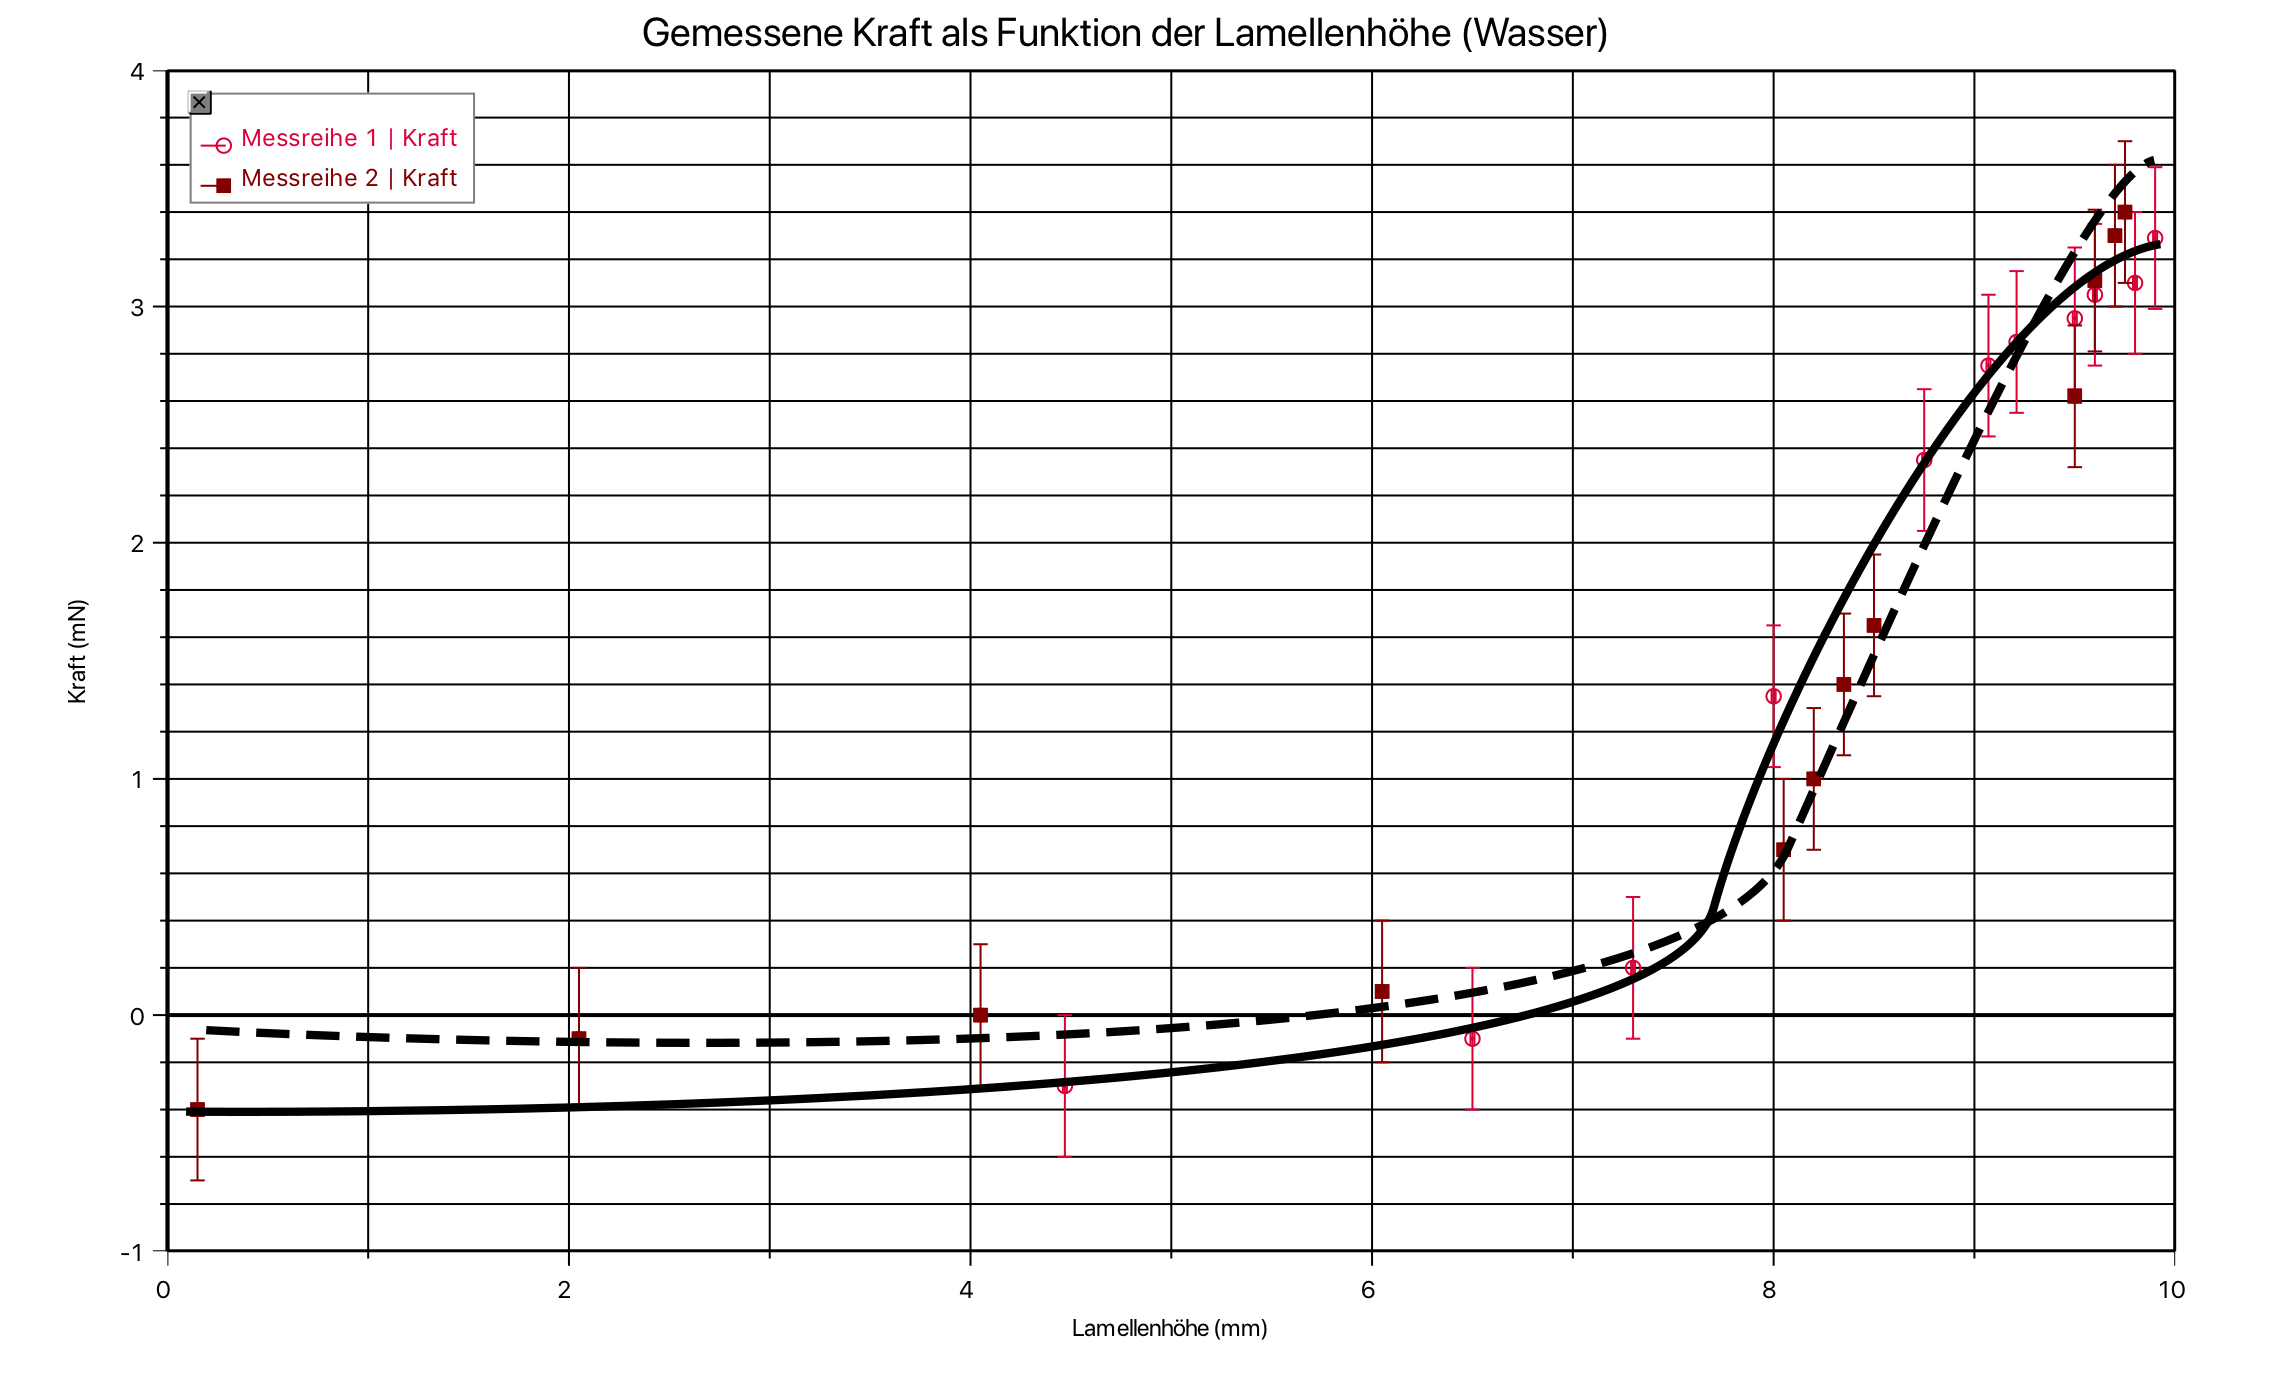
\includegraphics[width=\textwidth]{ex4gr1}
\caption{Verlauf der Kraft $F$ als Funktion der Lamellenhöhe sowie dessen Fit-Kurven bei Wasser.(Gepunktete Linie für die 2. Messreihe)}

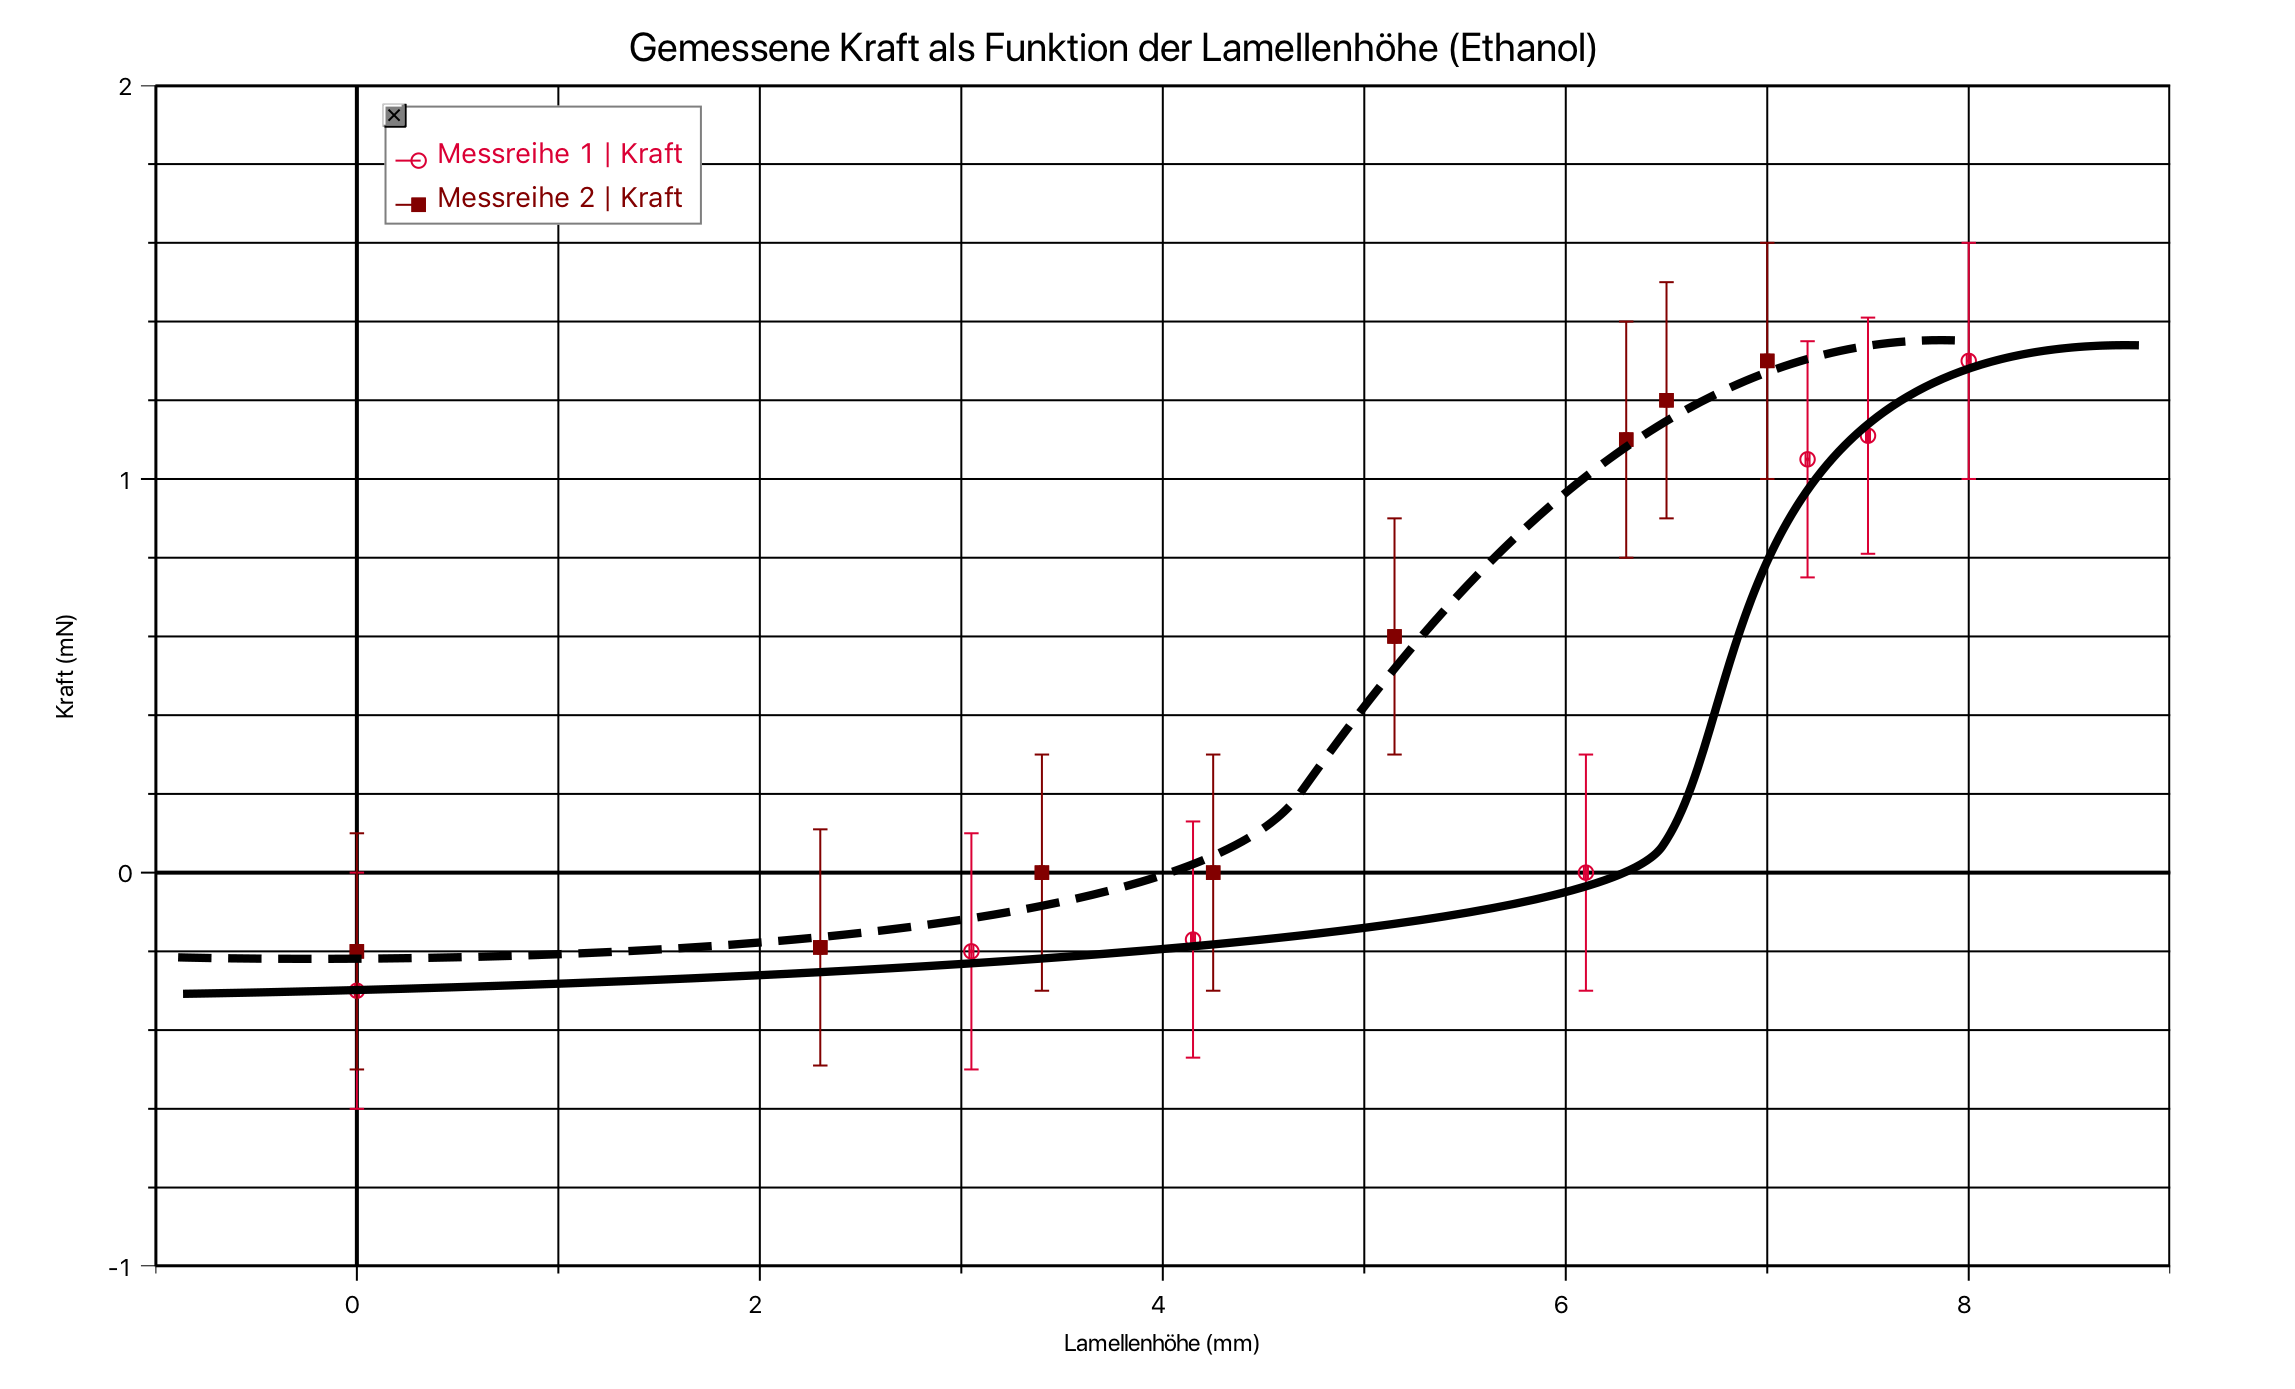
\includegraphics[width=\textwidth]{ex4gr2}
\caption{Verlauf der Kraft $F$ als Funktion der Lamellenhöhe sowie dessen Fit-Kurven bei Ethanol.(Gepunktete Linie für die 2. Messreihe)}
\end{figure}
\newpage

Die gemessene Länge des Messdrahtes war:
$$l=2,530 \pm 0,005 \textrm{cm}$$


Die einzelne $F(s_{\textrm{max}})$ wurden direkt von den Diagrammen mit den Fit-Kurven abgelesen, und deren Unsicherheiten als 0,3 \textrm{mN} genommen. Dadurch lassen sich die jeweiligen Oberflächenspannungen bestimmen. 


\begin{table}[h]
	\begin{tabular*}{0.99\textwidth}{@{\extracolsep{\fill}}cccccc}
		\toprule
		$F(s_{\textrm{max}})$ & $\Delta{F(s_{\textrm{max}})}$ & $\sigma$ & $\Delta\sigma$  \\
		mN & mN &  mN/cm & mN/cm   \\
		\midrule
		3,3 & 0,3 &  1,3 & 0,1 \\
		3,4 & 0,3 & 1,3 & 0,1 \\
		
		\bottomrule
	\end{tabular*}
	\caption{Kraft $F(s_\textrm{max})$ bei der maximalen Lamellenhöhe und die entsprechenden Oberflächenspannungen von Wasser}
	\label{tabelle5}
\end{table}

\begin{table}[h]
	\begin{tabular*}{0.99\textwidth}{@{\extracolsep{\fill}}cccccc}
		\toprule
		$F(s_{\textrm{max}})$ & $\Delta{F(s_{\textrm{max}})}$ & $\sigma$ & $\Delta\sigma$  \\
		mN & mN &  mN/cm & mN/cm   \\
		\midrule
		1,3 & 0,3 & 0,27  & 0,06 \\
		1,3 & 0,3 & 0,27 & 0,06 \\
		
		\bottomrule
	\end{tabular*}
	\caption{Kraft $F(s_\textrm{max})$ bei der maximalen Lamellenhöhe und die entsprechenden Oberflächenspannungen von Ethanol}
	\label{tabelle6}
\end{table}
 
Für die Berechnung der Unsicherheiten wurde die vereinfachte Formel für Produkte und Quotienten benutzt. Das Berechnungsverfahren ist genau wie in dem 1. Teil dargestellt. 
Die Mittelwerte und ihre Unsicherheiten lauten (Siehe Tabelle 7):


\begin{table}[h]
	\begin{tabular*}{0.99\textwidth}{@{\extracolsep{\fill}}cccccc}
		\toprule
		$\overline{\sigma}_{\textrm{Wasser}}$ & $u_{\overline{\sigma}\textrm{Wasser}}$ & $\overline{\sigma}_{\textrm{Ethanol}}$ & $\Delta\overline{\sigma}_{\textrm{Ethanol}}*$  \\
		mN & mN &  mN/cm & mN/cm   \\
		\midrule
		1,32 & 0,03 & 0,26  & 0,04 \\
		
		\bottomrule
	\end{tabular*}
	\caption{Die Mittelwerte der berechneten Oberflächenspannungen in Wasser und Ethanol und ihre Unsicherheiten.}
	\label{tabelle7}
\end{table}
*Da die gemessene Oberflächenspannungen für beide Messreihen dieselben Werte hatten, wurde die statistische Unsicherheit der Einzelmessung mit einer Skalierung für Mehrfachmessungen (nämlich $\frac{1}{\sqrt{2}}$) benutzt.

\section{Diskussion der Ergebnisse}
\subsection{1. Versuchsteil}
Die mit der Jolly'schen Federwaage gemessenen Dichte des Zylinders ist:
$$(1160\pm 70)\textrm{kg/m}^3$$
und die durch Gewicht- und Volumenmessungen bestimmte Dichte:
$$(1170\pm 50)\textrm{kg/m}^3$$
Da beide Werte innerhalb ihrer Unsicherheiten liegen, stimmen beide Werte überein. 

Die berechnete Dichte der unbekannten Flüssigkeit ist:
$$(750 \pm 70) \textrm{kg/m}^3$$

Ein möglicher Systematischer Fehler könnte sein, dass die Messungen mit einem nicht idealen Feder durchgeführt wurden. Deshalb könnte es Abweichungen von der linearen Beziehung zwischen Kraft und Abstand geben. In diesem Fall sind die benutzten Formeln von schlechten Modellen und liefern falsche Ergebnisse. 

Eine statistische Unsicherheit ist die Dicke der horizontalen Komponente der Waage, mit der die Höhe der Schalen abgelesen werden kann. Die Dicke könnte zu einer Ungenauigkeit von dem Ablesen von den Auslenkungen $x_0$, $x_1$ usw. auf der Skala führen. Dieses Problem lässt sich dadurch lösen, indem man diese Komponente dünner macht. 

Der Schutz der Feder vor äußeren Faktoren wie grosse 
Temperaturwechsel, Luftfeuchtigkeit und extreme mechanische Kräfte sind mögliche Lösungen. Die Herstellung der Feder aus widerstandsfähigen Materiellen, die von diesen Faktoren nicht leicht beeinträchtigt werden, ist auch eine Lösung. 

In dem 2. Teil ist auch ein Systematischer Fehler zu berücksichtigen. Aufgrund der Unsicherheit der Dichtmessung in dem 1. Versuchsteil können die berechneten Werten zu hoch oder zu klein abgeschätzt worden sein.

\subsection{2. Versuchsteil}
Es wurde berechnet, dass die Oberflächenspannung von Wasser ist:
$$(1,32\pm 0,03) \textrm{mN/cm}$$
und die von Ethanol:
$$(0,257 \pm 0,04) \textrm{mN/cm}$$

Die Literaturwerte für die Oberflächenspannungen von Wasser und Ethanol sind:
$$\gamma_W = 0,7199 \textrm{mN cm}^{-1}$$
$$\gamma_{Et} = 0,2235 \textrm{mN cm}^{-1}$$
(,,Surface-Tension Values.'').
Die Abweichungen zwischen den Literaturwerten und den gemessenen Werten in Einheiten der Standardunsicherheiten sind:
$$ t_W \approx 20 $$
$$ t_{Et} \approx 0,84$$

Es kann leicht gesehen werden, dass das Ergebnis für die Oberflächenspannung von Wasser nicht mit dem Literatur verträglich ist, da die Abweichung viel größer als zwei Standardunsicherheiten ist. Das Ergebnis für Ethanol ist aber mit dem Literaturwert Verträglich, da ihre Differenz kleiner als zwei Standardabweichungen ist. Mögliche Gründe dafür wird unten diskutiert.


Eine große Systematische Unsicherheit war es, dass  $F(s_\textrm{max})$ nicht direkt bestimmt werden konnte. Die letzten Messwerte sind die Werte, die gemessen wurden, bevor die Lamelle gerissen war. Das heißt, die letzten Datenpunkte liegen alle unter dem wirklichen $F(s_\text{max})$. Zusätzlich ist ein statistischer Fehler, dass die Werte für $F(s_\textrm{max})$ von einer selbst gezeichneten Kurve abgeschätzt werden mussten. Es können mehrere Kurven geben, die mit den Datenmessungen passen, und je nach dem, wie man die Kurven zeichnen, können die abgelesenen Werte für $F(s_\textrm{max})$ anders sein. Beide Probleme lassen sich dadurch verbessern, indem man die Mikrometerschraube langsamer dreht und Messungen häufiger macht. 

\newpage
\section{Anhang: Rohe Daten}
\subsection{1. Versuchsteil}
\begin{table}[h]
	\begin{tabular*}{0.99\textwidth}{@{\extracolsep{\fill}}cccccc}
		\toprule
		$x_1$ & $x_2$ &  $x_0$    \\
		mm & mm &  mm    \\
		\midrule
		395 & 409 & 412 \\
		441 & 457 &  460 \\
		412 &  430 & 432  \\
		402 & 418 & 420 \\
		
		\bottomrule
	\end{tabular*}
	\caption{Gemessene Werte für $x_1$, $x_2$ und $x_0$ (1. Teil)}
	\label{tabelle}
\end{table}
\begin{table}[h]
	\begin{tabular*}{0.99\textwidth}{@{\extracolsep{\fill}}cccccc}
		\toprule
		$x_1$ & $x_2$ &  $x_0$    \\
		mm & mm &  mm    \\
		\midrule
		391 & 404 & 411 \\
		384 & 396 &  403 \\
		413 &  425 & 432  \\
		440 & 453 & 459 \\
		
		\bottomrule
	\end{tabular*}
	\caption{Gemessene Werte für $x_1$, $x_2$ und $x_0$ (2. Teil)}
	\label{tabelle}
\end{table}

Alle Unsicherheiten sind $\pm$ 1mm. 

\subsection{2. Versuchsteil}
Da die Tabellen zu lang sind, bitte siehe Zusatzblätter für die rohen Daten zum 2. Versuchsteil. 


%lots of problems with the Jollysche Federwaage. Statis:The Feder may not be 
%System: The Kraft may not be linear. The condition of the spring may affect its performance. (Such as geometrical deformation from perfect circle). Einfluss der Federkonstante (nichtidealer Feder) nach Länge. Formula may not reflect real force.


\newpage
\section{Literatur}
,,Dichte.''\space Wikipedia.

,,Surface-tension Values.'' \space Wikipedia.

,,Versuchseinleitungen zum Physiklabor für Anfänger*innen, Teil 1.'' \space  Albert-Ludwigs-Universität Freiburg, 2018. 



\end{document}